\documentclass{article}
\usepackage[utf8]{inputenc}
\usepackage[russian]{babel}
\usepackage{csquotes}
\title{Обзор современных методов сегментации изображений.}
\author{Руденко Ирина, группа М05-894а.}
\date{18 декабря 2018}

\usepackage{natbib}
\usepackage{graphicx}

\begin{document}

\maketitle

\section{Постановка задачи.}
\textbf{Сегментация} — это хорошо известная задача компьютерного зрения, одна из трех важнейших, наряду с классификацией и обнаружением объектов. Задача сегментации изображений заключается в разделении изображения на фрагменты(группы пикселов) по определённому критерию. Существуют различные критерии: выделение общего объекта на изображении(ко-сегментация); выделение указанного пользователем объекта(извлечение объекта); разделение изображения на регионы, сходные по своему содержанию, но различимые визуально от соседей(сегментация без учителя). В своей работе я хочу обратить внимание на современные подходы в задаче семантическоой сегментации.

\textbf{Семантическая сегментация} - это попиксельная классификация изображения, где каждая метка соответствует определённому объекту. Так как цвета и яркости различных групп пикселей могут значительно отличаться, то сегментационной модели необходимо продемонстрировать некоторое \textquote{понимание} изображение, объединяя близкие по яркости, цвету, текстуре окрестности кусочки в \textquote{семантически} единый сегмент изображения.

\begin{figure}[h!]
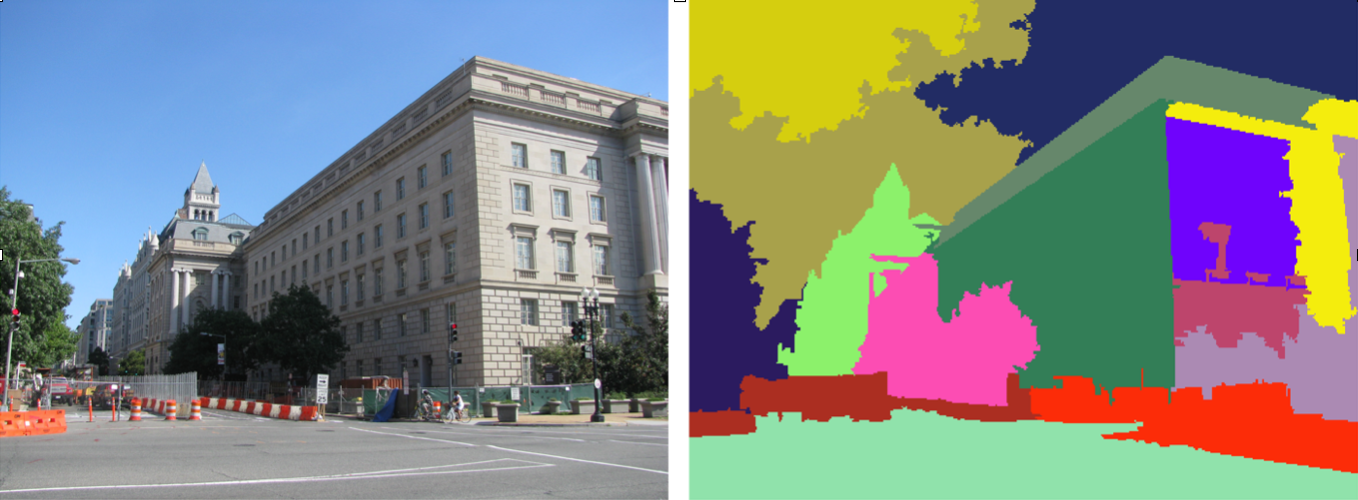
\includegraphics[width=\linewidth]{seg1.png}
\caption{Пример семантической сегментации.}
\end{figure}

Методы оценки качества сегментации должны включать оценку соответствия границ сегментов границам объектов и вложения объекта в сегмент. Используются классификационные метрики: accuracy, precision, recall, f-мера. Также существует метрика Intersection over Union (IoU), которая расчитывается для каждого класса как частное области перекрытия и области объединения.


\begin{table}[]
\centering
    \centering
    \begin{tabular}{c c}
        $IoU(i) = \frac{|X_i \cap Y_i|}{|X_i \cup Y_i|}$ &  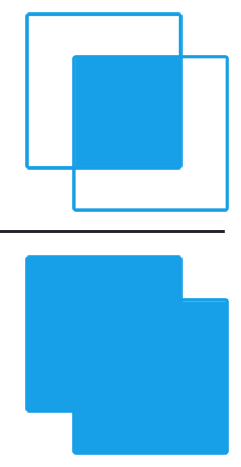
\includegraphics[scale=0.2, angle=90]{iou_equation.png}
    \end{tabular}
\end{table}


\section{Методы семантической сегментации изображений.}
Рассмотрим наиболее популярные подходы. 

\subsection{Независимая попиксельная классификация.}
Самый простой и очевидный подход - это классификационная модель. В таком случае метка класса определяется для каждого пиксела: задача рассматривается как задача \textquote{попиксельной} классификаци. Например, использование классических классификационных нейросетей и подавать им на вход некоторую окрестность классифицируемого пикселя. Точность сегментации повышается с увеличением размера окна, так как оно охватывает больше контекстной информации, при этом увеличивается перекрытие соседних окон, таким образом возрастает объем избыточных вычислений. Основным недостатком подхода является вычислительная сложность алгоритма, а соответственно низкая скорость работы.
\subsection{Полносвёрточные нейронные сети.}
Идея заключается в использовании Fully-convolutional нейронных сетей, построенных из AlexNet, VGG или GoogLeNet \cite{long_fully_2015}.
\noindent\begin{minipage}{0.6\textwidth}
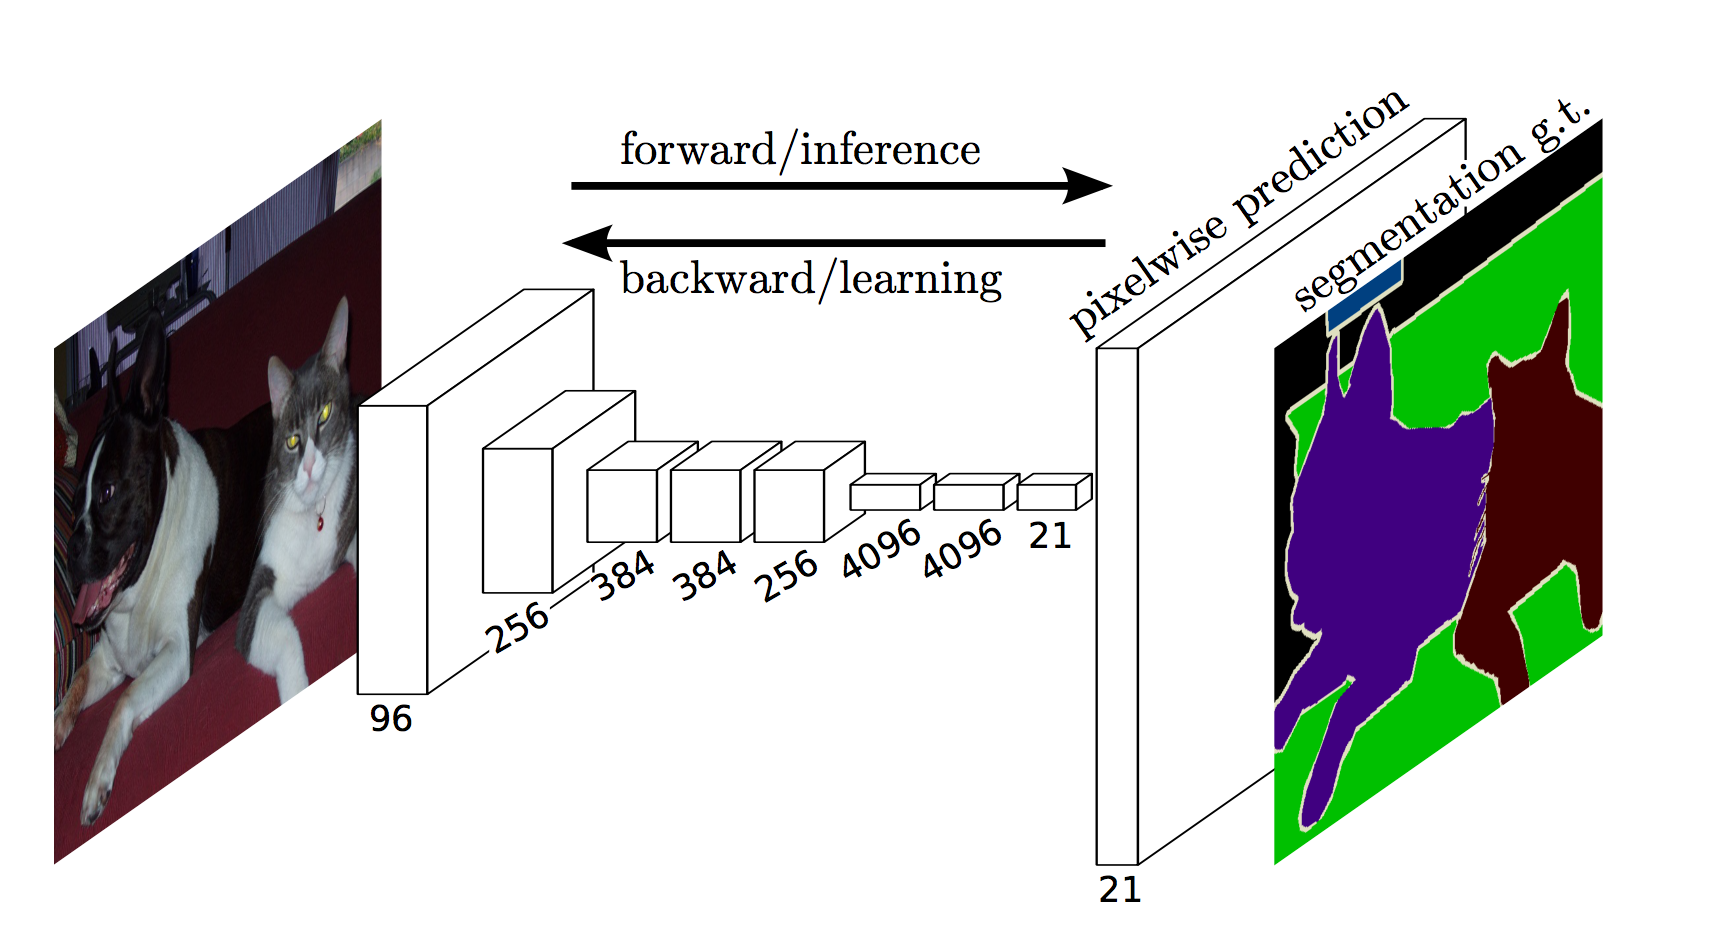
\includegraphics[width=\linewidth]{fc.png}}
\end{minipage}
\begin{minipage}{0.4\textwidth}
Для построения соответсвующей сети необходимо обрезать последние слои исходной и добавить слой up-conv для получения карты с вероятностями классов. 
\end{minipage}
Этот подход позволяет эффективно(без избыточных вычислений) получить высокое качество поточечной классификации.

\subsection{Графические модели: CRF(Conditional random fields).}
Также существует метод уточнения границ, при котором результат какого-либо классификатора улучшают с помощью графических моделей. Предлагаю рассмотреть один из подходов из статьи про CRF\cite{shotton_textonboost:_2006}. Условное случайное поле (Conditional Random Field, CRF) — это статистический метод классификации, характерным отличием которого является возможность учитывать «контекст» классифицируемого объекта. На множестве классифицируемых объектов необходимо построить граф смежности с заданными унарными и парными потенциалами, где унарные потенциалы - это вероятность класса, а парный потенциал задаёт эвристику оценивающую вероятность того, что два смежных объекта принадлежат одному классу.

\begin{figure}[h!]
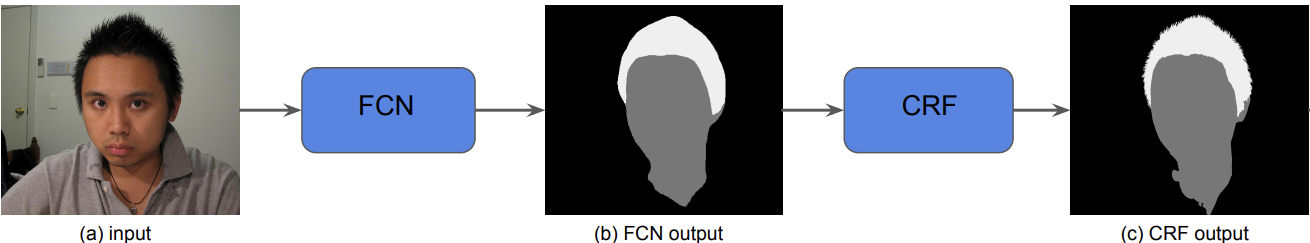
\includegraphics[width=\linewidth]{crf.png}
\caption{Использоование CRF для уточнения границ.}
\end{figure}

Далее вычисляется распределение $p(y| x)$(вероятности метки при условии вероятности класса объекта и контекста) как сумма парных потенциалов по всем смежным вершинам и унарного потенциала в точке, после чего задача предсказания состоит в том, чтобы оптимальным образом восстановить значения y, при условии, что нам даны наблюдаемые x, соответственно найти $argmax_y p(y| x)$(вероятности метки при условии вероятности класса объекта и контекста). 

Унарные потенциалы задаются, например, как выходы классификаторов и шкалируются так, чтобы выходы лежали в $[0,1]$  Парные потенциалы могут состоять из: нормы разности интенсивности, штрафа за разные метки смежных пикселей.

\subsection{Полносвёрточные encoder-decoder нейронные сети.}
Другим популярным подходом являются encoder-decoder сегментацинные сети\cite{badrinarayanan_segnet:_2015}. Основа работы полносвёрточных сетей – свёртка изображения. Пройдя через требуемое количество слоёв свёртки, изображение затем попадает в слои пулинга  и регуляризации. После экспериментально выясненного количество блоков downsampling-а уменьшенное изображение требуется вернуть к изначальному размеру. Слой upsample (upsample layer) выполняет увеличение изображения. На каждый выход имеется два входных изображения: первое – это обработанная картинка с предыдущего слоя (это может быть convolution или pooling), второе – это картинка из соответствующий pooling layer.  

\begin{figure}[h!]
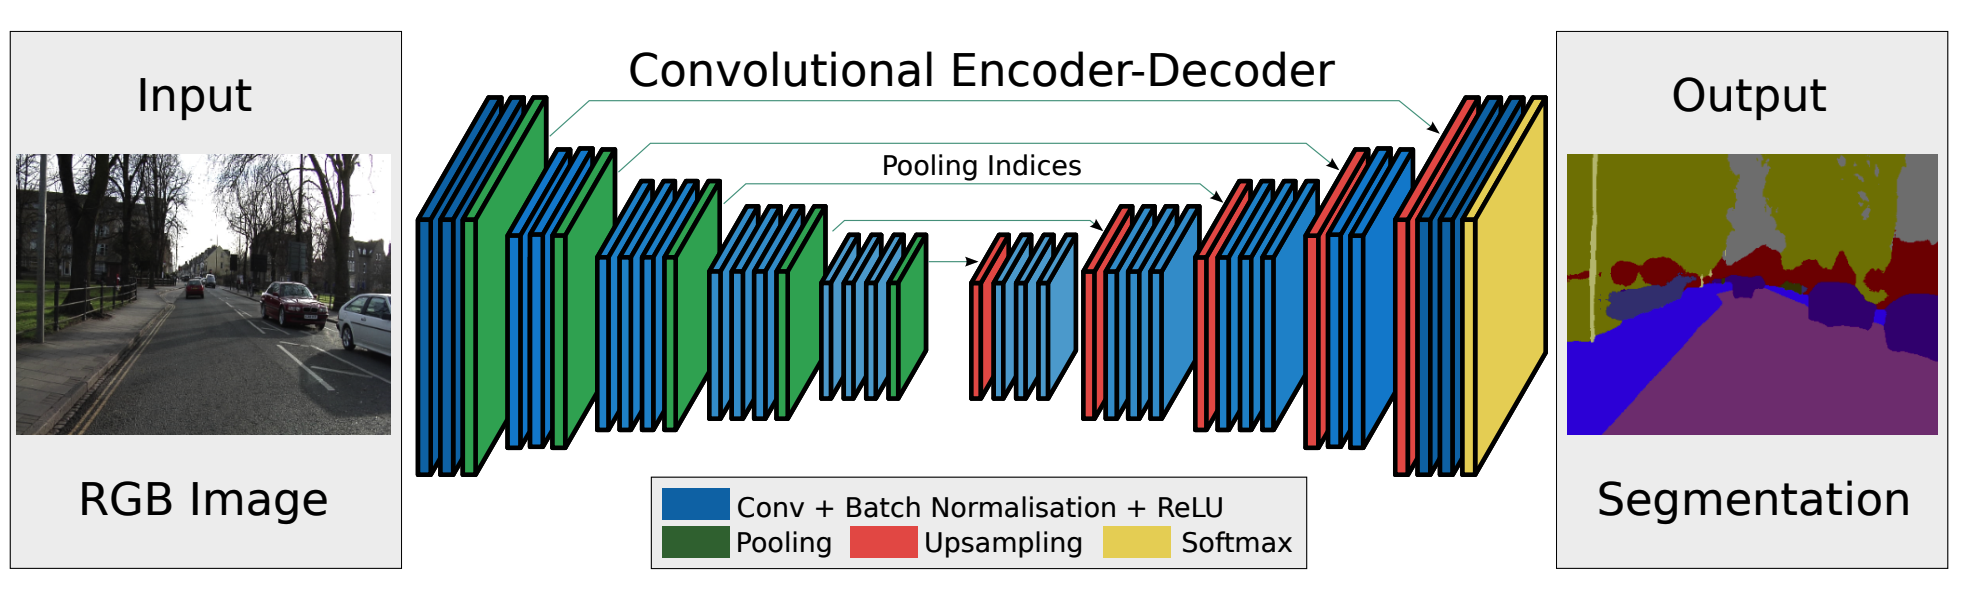
\includegraphics[width=\linewidth]{ed.png}
\caption{Архитектура Segnet.}
\end{figure}

\subsection{Заключение.}
Большое разнообразие подходов и архитектур для задачи семантической сегментации позволяет решать значимые прикладные задачи, находя оптимальное соотношение качества сегментации против вычислительной сложности алгоритма. Оптимальным выбором для многих приложений сейчас считаются encoder-decoder CNN.

\bibliographystyle{abbrv}
\bibliography{CV.bib}
\end{document}
